% =====================================================================
%  DORI signal-chain blocks, corrected export of your mathcha drawing.
%  Nothing of yours was modified; this is a separate file.
%
%  WHAT WAS CHANGED, and nothing else:
%
%  1. One command per line. Pasted as a single line, the first % comment
%     swallows the whole picture and you get an empty page.
%
%  2. Grey arrows centred on the boxes. The boxes run x 220 -> 283.04,
%     so their centre is x = 251.52; the arrows were at x = 254.45.
%     They now start exactly on the bottom edge of one box (y 228.67,
%     y 259.42) and end exactly on the top edge of the next (y 236.12,
%     y 266.87).
%
%  3. Waveform baselines levelled. Each baseline now sits on the same y
%     as the bottom edge of its box (228.67 / 259.42 / 290.16), all three
%     start at x 294.07 and end at x 331.84 with the arrowhead at 334.84.
%     The curves and plateaux that rest on them were moved to match.
%
%  4. Block labels. Mathcha writes them as \textbf{{\tiny ...}}\\ inside a
%     minipage, so the \\ uses the outer 12 pt baselineskip while the text
%     is 5 pt: the two lines fly apart and out of the shapes. Each label is
%     now one centred node on the box centre, at 4.5 pt on 5.4 pt leading
%     (set by "Discrimination", the widest word), coloured like its box.
%
%  5. "N Bin \ E" -> $N_{\mathrm{bin}} \propto E$, moved to (298.00,292.60)
%     so it clears the baseline arrow instead of sitting on it.
%
%  Use it exactly like your other figure files:
%      \resizebox{\linewidth}{!}{% =====================================================================
%  DORI signal-chain blocks, corrected export of your mathcha drawing.
%  Nothing of yours was modified; this is a separate file.
%
%  WHAT WAS CHANGED, and nothing else:
%
%  1. One command per line. Pasted as a single line, the first % comment
%     swallows the whole picture and you get an empty page.
%
%  2. Grey arrows centred on the boxes. The boxes run x 220 -> 283.04,
%     so their centre is x = 251.52; the arrows were at x = 254.45.
%     They now start exactly on the bottom edge of one box (y 228.67,
%     y 259.42) and end exactly on the top edge of the next (y 236.12,
%     y 266.87).
%
%  3. Waveform baselines levelled. Each baseline now sits on the same y
%     as the bottom edge of its box (228.67 / 259.42 / 290.16), all three
%     start at x 294.07 and end at x 331.84 with the arrowhead at 334.84.
%     The curves and plateaux that rest on them were moved to match.
%
%  4. Block labels. Mathcha writes them as \textbf{{\tiny ...}}\\ inside a
%     minipage, so the \\ uses the outer 12 pt baselineskip while the text
%     is 5 pt: the two lines fly apart and out of the shapes. Each label is
%     now one centred node on the box centre, at 4.5 pt on 5.4 pt leading
%     (set by "Discrimination", the widest word), coloured like its box.
%
%  5. "N Bin \ E" -> $N_{\mathrm{bin}} \propto E$, moved to (298.00,292.60)
%     so it clears the baseline arrow instead of sitting on it.
%
%  Use it exactly like your other figure files:
%      \resizebox{\linewidth}{!}{% =====================================================================
%  DORI signal-chain blocks, corrected export of your mathcha drawing.
%  Nothing of yours was modified; this is a separate file.
%
%  WHAT WAS CHANGED, and nothing else:
%
%  1. One command per line. Pasted as a single line, the first % comment
%     swallows the whole picture and you get an empty page.
%
%  2. Grey arrows centred on the boxes. The boxes run x 220 -> 283.04,
%     so their centre is x = 251.52; the arrows were at x = 254.45.
%     They now start exactly on the bottom edge of one box (y 228.67,
%     y 259.42) and end exactly on the top edge of the next (y 236.12,
%     y 266.87).
%
%  3. Waveform baselines levelled. Each baseline now sits on the same y
%     as the bottom edge of its box (228.67 / 259.42 / 290.16), all three
%     start at x 294.07 and end at x 331.84 with the arrowhead at 334.84.
%     The curves and plateaux that rest on them were moved to match.
%
%  4. Block labels. Mathcha writes them as \textbf{{\tiny ...}}\\ inside a
%     minipage, so the \\ uses the outer 12 pt baselineskip while the text
%     is 5 pt: the two lines fly apart and out of the shapes. Each label is
%     now one centred node on the box centre, at 4.5 pt on 5.4 pt leading
%     (set by "Discrimination", the widest word), coloured like its box.
%
%  5. "N Bin \ E" -> $N_{\mathrm{bin}} \propto E$, moved to (298.00,292.60)
%     so it clears the baseline arrow instead of sitting on it.
%
%  Use it exactly like your other figure files:
%      \resizebox{\linewidth}{!}{% =====================================================================
%  DORI signal-chain blocks, corrected export of your mathcha drawing.
%  Nothing of yours was modified; this is a separate file.
%
%  WHAT WAS CHANGED, and nothing else:
%
%  1. One command per line. Pasted as a single line, the first % comment
%     swallows the whole picture and you get an empty page.
%
%  2. Grey arrows centred on the boxes. The boxes run x 220 -> 283.04,
%     so their centre is x = 251.52; the arrows were at x = 254.45.
%     They now start exactly on the bottom edge of one box (y 228.67,
%     y 259.42) and end exactly on the top edge of the next (y 236.12,
%     y 266.87).
%
%  3. Waveform baselines levelled. Each baseline now sits on the same y
%     as the bottom edge of its box (228.67 / 259.42 / 290.16), all three
%     start at x 294.07 and end at x 331.84 with the arrowhead at 334.84.
%     The curves and plateaux that rest on them were moved to match.
%
%  4. Block labels. Mathcha writes them as \textbf{{\tiny ...}}\\ inside a
%     minipage, so the \\ uses the outer 12 pt baselineskip while the text
%     is 5 pt: the two lines fly apart and out of the shapes. Each label is
%     now one centred node on the box centre, at 4.5 pt on 5.4 pt leading
%     (set by "Discrimination", the widest word), coloured like its box.
%
%  5. "N Bin \ E" -> $N_{\mathrm{bin}} \propto E$, moved to (298.00,292.60)
%     so it clears the baseline arrow instead of sitting on it.
%
%  Use it exactly like your other figure files:
%      \resizebox{\linewidth}{!}{\input{architecture_blocks.tex}}
%  Needs only \usepackage{tikz}, which the poster already loads.
% =====================================================================

\tikzset{every picture/.style={line width=0.75pt}}
%set default line width to 0.75pt 
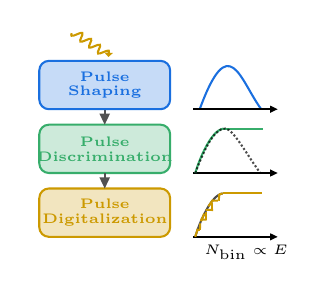
\begin{tikzpicture}[x=0.75pt,y=0.75pt,yscale=-1,xscale=1]
%uncomment if require: \path (0,623);
%set diagram left start at 0, and has height of 623
%Curve Lines [id:da31175352604231354]
\draw [color={rgb, 255:red, 26; green, 111; blue, 223 } ,draw opacity=1 ] (297.29,228.67) .. controls (311.48,189.89) and (316.58,214.56) .. (326.94,228.67) ;
%Straight Lines [id:da8734375505712497]
\draw (294.07,228.67) -- (331.84,228.67) ;
\draw [shift={(334.84,228.67)}, rotate = 180] [fill={rgb, 255:red, 0; green, 0; blue, 0 } ][line width=0.08] [draw opacity=0] (3.57,-1.72) -- (0,0) -- (3.57,1.72) -- cycle ;
%Straight Lines [id:da44513384727711636]
\draw (294.07,290.16) -- (331.84,290.16) ;
\draw [shift={(334.84,290.16)}, rotate = 180] [fill={rgb, 255:red, 0; green, 0; blue, 0 } ][line width=0.08] [draw opacity=0] (3.57,-1.72) -- (0,0) -- (3.57,1.72) -- cycle ;
%Curve Lines [id:da06577028557977793]
\draw [color={rgb, 255:red, 0; green, 0; blue, 0 } ,draw opacity=0.7 ] (295.15,290.16) .. controls (296.85,284.16) and (302.58,269.99) .. (308.33,269.24) ;
%Straight Lines [id:da0572237289311508]
\draw [color={rgb, 255:red, 0; green, 0; blue, 0 } ,draw opacity=0.7 ] (308.33,269.24) -- (327.15,269.24) ;
%Curve Lines [id:da3804043288541633]
\draw [color={rgb, 255:red, 204; green, 153; blue, 0 } ,draw opacity=1 ] [dash pattern={on 3pt off 3pt on 3pt off 3pt}] (295.15,290.16) .. controls (296.85,284.16) and (302.58,269.99) .. (308.33,269.24) ;
%Straight Lines [id:da5333998307295363]
\draw [color={rgb, 255:red, 204; green, 153; blue, 0 } ,draw opacity=1 ] (295.76,286.75) -- (297.39,286.83) ;
%Straight Lines [id:da40393427405433224]
\draw [color={rgb, 255:red, 204; green, 153; blue, 0 } ,draw opacity=1 ] (297.39,286.83) -- (297.49,283.65) ;
%Straight Lines [id:da7440185216718632]
\draw [color={rgb, 255:red, 204; green, 153; blue, 0 } ,draw opacity=1 ] (303.28,272.68) -- (305.99,272.69) ;
%Straight Lines [id:da4575813772961881]
\draw [color={rgb, 255:red, 204; green, 153; blue, 0 } ,draw opacity=1 ] (306.47,272.78) -- (306.7,269.62) ;
%Straight Lines [id:da012864593156911797]
\draw [color={rgb, 255:red, 204; green, 153; blue, 0 } ,draw opacity=1 ] (297.68,281.8) -- (300.65,281.85) ;
%Straight Lines [id:da7563678124476333]
\draw [color={rgb, 255:red, 204; green, 153; blue, 0 } ,draw opacity=1 ] (300.13,281.96) -- (300.13,278.31) ;
%Straight Lines [id:da5333243365793827]
\draw [color={rgb, 255:red, 204; green, 153; blue, 0 } ,draw opacity=1 ] (301,277.21) -- (300.2,277.18) -- (303.71,277.22) ;
%Straight Lines [id:da6175946543817453]
\draw [color={rgb, 255:red, 204; green, 153; blue, 0 } ,draw opacity=1 ] (303.06,277.27) -- (303.06,276.8) -- (303.06,276.78) -- (303.06,273.62) ;
%Straight Lines [id:da3521344691026579]
\draw [color={rgb, 255:red, 204; green, 153; blue, 0 } ,draw opacity=1 ] (308.33,269.24) -- (327.15,269.24) ;
%Shape: Wave [id:dp9368433800430482]
\draw [color={rgb, 255:red, 204; green, 153; blue, 0 } ,draw opacity=1 ] (235.61,192.06) .. controls (235.39,192.63) and (235.3,193.09) .. (235.56,193.27) .. controls (235.94,193.52) and (237.01,193.07) .. (238.13,192.59) .. controls (239.24,192.11) and (240.31,191.66) .. (240.7,191.91) .. controls (241.08,192.17) and (240.68,193.07) .. (240.25,194.02) .. controls (239.83,194.96) and (239.43,195.86) .. (239.81,196.12) .. controls (240.2,196.38) and (241.26,195.92) .. (242.38,195.45) .. controls (243.5,194.97) and (244.57,194.51) .. (244.95,194.77) .. controls (245.34,195.03) and (244.94,195.93) .. (244.51,196.87) .. controls (244.09,197.82) and (243.68,198.72) .. (244.07,198.98) .. controls (244.45,199.24) and (245.52,198.78) .. (246.64,198.3) .. controls (247.76,197.82) and (248.82,197.37) .. (249.21,197.63) .. controls (249.59,197.88) and (249.19,198.78) .. (248.77,199.73) .. controls (248.34,200.67) and (247.94,201.58) .. (248.33,201.83) .. controls (248.71,202.09) and (249.78,201.64) .. (250.9,201.16) .. controls (252.01,200.68) and (253.08,200.22) .. (253.47,200.48) .. controls (253.82,200.72) and (253.51,201.51) .. (253.12,202.37) ;
%Shape: Triangle [id:dp9985044017508556]
\draw [color={rgb, 255:red, 204; green, 153; blue, 0 } ,draw opacity=1 ][fill={rgb, 255:red, 204; green, 153; blue, 0 } ,fill opacity=1 ] (253.35,202.81) -- (252.57,201.95) -- (254.24,202.02) -- cycle ;
%Rounded Rect [id:dp19934922796405263]
\draw [color={rgb, 255:red, 55; green, 173; blue, 107 } ,draw opacity=1 ][fill={rgb, 255:red, 55; green, 173; blue, 107 } ,fill opacity=0.25 ] (220,240.78) .. controls (220,238.21) and (222.09,236.12) .. (224.66,236.12) -- (278.38,236.12) .. controls (280.95,236.12) and (283.04,238.21) .. (283.04,240.78) -- (283.04,254.76) .. controls (283.04,257.33) and (280.95,259.42) .. (278.38,259.42) -- (224.66,259.42) .. controls (222.09,259.42) and (220,257.33) .. (220,254.76) -- cycle ;
%Straight Lines [id:da15405365263406912]
\draw [color={rgb, 255:red, 81; green, 81; blue, 81 } ,draw opacity=1 ] (251.52,228.67) -- (251.52,233.12) ;
\draw [shift={(251.52,236.12)}, rotate = 270] [fill={rgb, 255:red, 81; green, 81; blue, 81 } ,fill opacity=1 ][line width=0.08] [draw opacity=0] (5.36,-2.57) -- (0,0) -- (5.36,2.57) -- cycle ;
%Rounded Rect [id:dp9679678320320008]
\draw [color={rgb, 255:red, 26; green, 111; blue, 223 } ,draw opacity=1 ][fill={rgb, 255:red, 26; green, 111; blue, 223 } ,fill opacity=0.25 ] (220,210.03) .. controls (220,207.46) and (222.09,205.37) .. (224.66,205.37) -- (278.38,205.37) .. controls (280.95,205.37) and (283.04,207.46) .. (283.04,210.03) -- (283.04,224.01) .. controls (283.04,226.58) and (280.95,228.67) .. (278.38,228.67) -- (224.66,228.67) .. controls (222.09,228.67) and (220,226.58) .. (220,224.01) -- cycle ;
%Rounded Rect [id:dp4047477037578918]
\draw [color={rgb, 255:red, 204; green, 153; blue, 0 } ,draw opacity=1 ][fill={rgb, 255:red, 204; green, 153; blue, 0 } ,fill opacity=0.25 ] (220,271.53) .. controls (220,268.96) and (222.09,266.87) .. (224.66,266.87) -- (278.38,266.87) .. controls (280.95,266.87) and (283.04,268.96) .. (283.04,271.53) -- (283.04,285.51) .. controls (283.04,288.08) and (280.95,290.16) .. (278.38,290.16) -- (224.66,290.16) .. controls (222.09,290.16) and (220,288.08) .. (220,285.51) -- cycle ;
%Straight Lines [id:da0010432308854115835]
\draw (294.07,259.42) -- (331.84,259.42) ;
\draw [shift={(334.84,259.42)}, rotate = 180] [fill={rgb, 255:red, 0; green, 0; blue, 0 } ][line width=0.08] [draw opacity=0] (3.57,-1.72) -- (0,0) -- (3.57,1.72) -- cycle ;
%Curve Lines [id:da4874347648440388]
\draw [color={rgb, 255:red, 55; green, 173; blue, 107 } ,draw opacity=1 ] (295.17,259.42) .. controls (296.91,253.15) and (302.75,238.82) .. (308.61,238.06) ;
%Straight Lines [id:da23704226954075758]
\draw [color={rgb, 255:red, 55; green, 173; blue, 107 } ,draw opacity=1 ] (308.61,238.06) -- (327.80,238.06) ;
%Curve Lines [id:da042698988524645376]
\draw [color={rgb, 255:red, 0; green, 0; blue, 0 } ,draw opacity=0.7 ] [dash pattern={on 0.75pt off 0.75pt on 0.75pt off 0.75pt}] (295.17,259.42) .. controls (301.17,243.29) and (305.64,237.91) .. (309.53,237.99) .. controls (313.43,238.08) and (319.93,250.52) .. (326.49,259.42) ;
%Straight Lines [id:da33392936363629766]
\draw [color={rgb, 255:red, 81; green, 81; blue, 81 } ,draw opacity=1 ] (251.52,259.42) -- (251.52,263.87) ;
\draw [shift={(251.52,266.87)}, rotate = 270] [fill={rgb, 255:red, 81; green, 81; blue, 81 } ,fill opacity=1 ][line width=0.08] [draw opacity=0] (5.36,-2.57) -- (0,0) -- (5.36,2.57) -- cycle ;
% Text Node
\draw (298.00,292.60) node [anchor=north west][inner sep=0.75pt] [font=\tiny] [align=left] {$N_{\mathrm{bin}} \propto E$};
% Text Node
\draw (251.52,247.77) node [anchor=center, align=center, font=\fontsize{4.5}{5.4}\selectfont\bfseries, color={rgb, 255:red, 55; green, 173; blue, 107 }] {Pulse\\Discrimination};
% Text Node
\draw (251.52,217.02) node [anchor=center, align=center, font=\fontsize{4.5}{5.4}\selectfont\bfseries, color={rgb, 255:red, 26; green, 111; blue, 223 }] {Pulse\\Shaping};
% Text Node
\draw (251.52,278.51) node [anchor=center, align=center, font=\fontsize{4.5}{5.4}\selectfont\bfseries, color={rgb, 255:red, 204; green, 153; blue, 0 }] {Pulse\\Digitalization}; 


% Optional: label the incoming photon next to the yellow squiggle.
% Uncomment the next line if you want it.
%\draw (236.50,191.00) node [anchor=south east, font=\fontsize{4.5}{5.4}\selectfont, color={rgb, 255:red, 204; green, 153; blue, 0 }] {$h\nu$};
\end{tikzpicture}
}
%  Needs only \usepackage{tikz}, which the poster already loads.
% =====================================================================

\tikzset{every picture/.style={line width=0.75pt}}
%set default line width to 0.75pt 
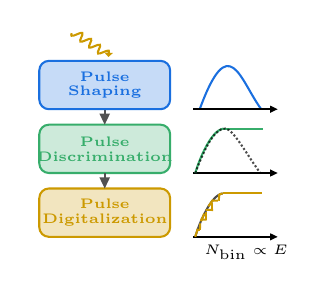
\begin{tikzpicture}[x=0.75pt,y=0.75pt,yscale=-1,xscale=1]
%uncomment if require: \path (0,623);
%set diagram left start at 0, and has height of 623
%Curve Lines [id:da31175352604231354]
\draw [color={rgb, 255:red, 26; green, 111; blue, 223 } ,draw opacity=1 ] (297.29,228.67) .. controls (311.48,189.89) and (316.58,214.56) .. (326.94,228.67) ;
%Straight Lines [id:da8734375505712497]
\draw (294.07,228.67) -- (331.84,228.67) ;
\draw [shift={(334.84,228.67)}, rotate = 180] [fill={rgb, 255:red, 0; green, 0; blue, 0 } ][line width=0.08] [draw opacity=0] (3.57,-1.72) -- (0,0) -- (3.57,1.72) -- cycle ;
%Straight Lines [id:da44513384727711636]
\draw (294.07,290.16) -- (331.84,290.16) ;
\draw [shift={(334.84,290.16)}, rotate = 180] [fill={rgb, 255:red, 0; green, 0; blue, 0 } ][line width=0.08] [draw opacity=0] (3.57,-1.72) -- (0,0) -- (3.57,1.72) -- cycle ;
%Curve Lines [id:da06577028557977793]
\draw [color={rgb, 255:red, 0; green, 0; blue, 0 } ,draw opacity=0.7 ] (295.15,290.16) .. controls (296.85,284.16) and (302.58,269.99) .. (308.33,269.24) ;
%Straight Lines [id:da0572237289311508]
\draw [color={rgb, 255:red, 0; green, 0; blue, 0 } ,draw opacity=0.7 ] (308.33,269.24) -- (327.15,269.24) ;
%Curve Lines [id:da3804043288541633]
\draw [color={rgb, 255:red, 204; green, 153; blue, 0 } ,draw opacity=1 ] [dash pattern={on 3pt off 3pt on 3pt off 3pt}] (295.15,290.16) .. controls (296.85,284.16) and (302.58,269.99) .. (308.33,269.24) ;
%Straight Lines [id:da5333998307295363]
\draw [color={rgb, 255:red, 204; green, 153; blue, 0 } ,draw opacity=1 ] (295.76,286.75) -- (297.39,286.83) ;
%Straight Lines [id:da40393427405433224]
\draw [color={rgb, 255:red, 204; green, 153; blue, 0 } ,draw opacity=1 ] (297.39,286.83) -- (297.49,283.65) ;
%Straight Lines [id:da7440185216718632]
\draw [color={rgb, 255:red, 204; green, 153; blue, 0 } ,draw opacity=1 ] (303.28,272.68) -- (305.99,272.69) ;
%Straight Lines [id:da4575813772961881]
\draw [color={rgb, 255:red, 204; green, 153; blue, 0 } ,draw opacity=1 ] (306.47,272.78) -- (306.7,269.62) ;
%Straight Lines [id:da012864593156911797]
\draw [color={rgb, 255:red, 204; green, 153; blue, 0 } ,draw opacity=1 ] (297.68,281.8) -- (300.65,281.85) ;
%Straight Lines [id:da7563678124476333]
\draw [color={rgb, 255:red, 204; green, 153; blue, 0 } ,draw opacity=1 ] (300.13,281.96) -- (300.13,278.31) ;
%Straight Lines [id:da5333243365793827]
\draw [color={rgb, 255:red, 204; green, 153; blue, 0 } ,draw opacity=1 ] (301,277.21) -- (300.2,277.18) -- (303.71,277.22) ;
%Straight Lines [id:da6175946543817453]
\draw [color={rgb, 255:red, 204; green, 153; blue, 0 } ,draw opacity=1 ] (303.06,277.27) -- (303.06,276.8) -- (303.06,276.78) -- (303.06,273.62) ;
%Straight Lines [id:da3521344691026579]
\draw [color={rgb, 255:red, 204; green, 153; blue, 0 } ,draw opacity=1 ] (308.33,269.24) -- (327.15,269.24) ;
%Shape: Wave [id:dp9368433800430482]
\draw [color={rgb, 255:red, 204; green, 153; blue, 0 } ,draw opacity=1 ] (235.61,192.06) .. controls (235.39,192.63) and (235.3,193.09) .. (235.56,193.27) .. controls (235.94,193.52) and (237.01,193.07) .. (238.13,192.59) .. controls (239.24,192.11) and (240.31,191.66) .. (240.7,191.91) .. controls (241.08,192.17) and (240.68,193.07) .. (240.25,194.02) .. controls (239.83,194.96) and (239.43,195.86) .. (239.81,196.12) .. controls (240.2,196.38) and (241.26,195.92) .. (242.38,195.45) .. controls (243.5,194.97) and (244.57,194.51) .. (244.95,194.77) .. controls (245.34,195.03) and (244.94,195.93) .. (244.51,196.87) .. controls (244.09,197.82) and (243.68,198.72) .. (244.07,198.98) .. controls (244.45,199.24) and (245.52,198.78) .. (246.64,198.3) .. controls (247.76,197.82) and (248.82,197.37) .. (249.21,197.63) .. controls (249.59,197.88) and (249.19,198.78) .. (248.77,199.73) .. controls (248.34,200.67) and (247.94,201.58) .. (248.33,201.83) .. controls (248.71,202.09) and (249.78,201.64) .. (250.9,201.16) .. controls (252.01,200.68) and (253.08,200.22) .. (253.47,200.48) .. controls (253.82,200.72) and (253.51,201.51) .. (253.12,202.37) ;
%Shape: Triangle [id:dp9985044017508556]
\draw [color={rgb, 255:red, 204; green, 153; blue, 0 } ,draw opacity=1 ][fill={rgb, 255:red, 204; green, 153; blue, 0 } ,fill opacity=1 ] (253.35,202.81) -- (252.57,201.95) -- (254.24,202.02) -- cycle ;
%Rounded Rect [id:dp19934922796405263]
\draw [color={rgb, 255:red, 55; green, 173; blue, 107 } ,draw opacity=1 ][fill={rgb, 255:red, 55; green, 173; blue, 107 } ,fill opacity=0.25 ] (220,240.78) .. controls (220,238.21) and (222.09,236.12) .. (224.66,236.12) -- (278.38,236.12) .. controls (280.95,236.12) and (283.04,238.21) .. (283.04,240.78) -- (283.04,254.76) .. controls (283.04,257.33) and (280.95,259.42) .. (278.38,259.42) -- (224.66,259.42) .. controls (222.09,259.42) and (220,257.33) .. (220,254.76) -- cycle ;
%Straight Lines [id:da15405365263406912]
\draw [color={rgb, 255:red, 81; green, 81; blue, 81 } ,draw opacity=1 ] (251.52,228.67) -- (251.52,233.12) ;
\draw [shift={(251.52,236.12)}, rotate = 270] [fill={rgb, 255:red, 81; green, 81; blue, 81 } ,fill opacity=1 ][line width=0.08] [draw opacity=0] (5.36,-2.57) -- (0,0) -- (5.36,2.57) -- cycle ;
%Rounded Rect [id:dp9679678320320008]
\draw [color={rgb, 255:red, 26; green, 111; blue, 223 } ,draw opacity=1 ][fill={rgb, 255:red, 26; green, 111; blue, 223 } ,fill opacity=0.25 ] (220,210.03) .. controls (220,207.46) and (222.09,205.37) .. (224.66,205.37) -- (278.38,205.37) .. controls (280.95,205.37) and (283.04,207.46) .. (283.04,210.03) -- (283.04,224.01) .. controls (283.04,226.58) and (280.95,228.67) .. (278.38,228.67) -- (224.66,228.67) .. controls (222.09,228.67) and (220,226.58) .. (220,224.01) -- cycle ;
%Rounded Rect [id:dp4047477037578918]
\draw [color={rgb, 255:red, 204; green, 153; blue, 0 } ,draw opacity=1 ][fill={rgb, 255:red, 204; green, 153; blue, 0 } ,fill opacity=0.25 ] (220,271.53) .. controls (220,268.96) and (222.09,266.87) .. (224.66,266.87) -- (278.38,266.87) .. controls (280.95,266.87) and (283.04,268.96) .. (283.04,271.53) -- (283.04,285.51) .. controls (283.04,288.08) and (280.95,290.16) .. (278.38,290.16) -- (224.66,290.16) .. controls (222.09,290.16) and (220,288.08) .. (220,285.51) -- cycle ;
%Straight Lines [id:da0010432308854115835]
\draw (294.07,259.42) -- (331.84,259.42) ;
\draw [shift={(334.84,259.42)}, rotate = 180] [fill={rgb, 255:red, 0; green, 0; blue, 0 } ][line width=0.08] [draw opacity=0] (3.57,-1.72) -- (0,0) -- (3.57,1.72) -- cycle ;
%Curve Lines [id:da4874347648440388]
\draw [color={rgb, 255:red, 55; green, 173; blue, 107 } ,draw opacity=1 ] (295.17,259.42) .. controls (296.91,253.15) and (302.75,238.82) .. (308.61,238.06) ;
%Straight Lines [id:da23704226954075758]
\draw [color={rgb, 255:red, 55; green, 173; blue, 107 } ,draw opacity=1 ] (308.61,238.06) -- (327.80,238.06) ;
%Curve Lines [id:da042698988524645376]
\draw [color={rgb, 255:red, 0; green, 0; blue, 0 } ,draw opacity=0.7 ] [dash pattern={on 0.75pt off 0.75pt on 0.75pt off 0.75pt}] (295.17,259.42) .. controls (301.17,243.29) and (305.64,237.91) .. (309.53,237.99) .. controls (313.43,238.08) and (319.93,250.52) .. (326.49,259.42) ;
%Straight Lines [id:da33392936363629766]
\draw [color={rgb, 255:red, 81; green, 81; blue, 81 } ,draw opacity=1 ] (251.52,259.42) -- (251.52,263.87) ;
\draw [shift={(251.52,266.87)}, rotate = 270] [fill={rgb, 255:red, 81; green, 81; blue, 81 } ,fill opacity=1 ][line width=0.08] [draw opacity=0] (5.36,-2.57) -- (0,0) -- (5.36,2.57) -- cycle ;
% Text Node
\draw (298.00,292.60) node [anchor=north west][inner sep=0.75pt] [font=\tiny] [align=left] {$N_{\mathrm{bin}} \propto E$};
% Text Node
\draw (251.52,247.77) node [anchor=center, align=center, font=\fontsize{4.5}{5.4}\selectfont\bfseries, color={rgb, 255:red, 55; green, 173; blue, 107 }] {Pulse\\Discrimination};
% Text Node
\draw (251.52,217.02) node [anchor=center, align=center, font=\fontsize{4.5}{5.4}\selectfont\bfseries, color={rgb, 255:red, 26; green, 111; blue, 223 }] {Pulse\\Shaping};
% Text Node
\draw (251.52,278.51) node [anchor=center, align=center, font=\fontsize{4.5}{5.4}\selectfont\bfseries, color={rgb, 255:red, 204; green, 153; blue, 0 }] {Pulse\\Digitalization}; 


% Optional: label the incoming photon next to the yellow squiggle.
% Uncomment the next line if you want it.
%\draw (236.50,191.00) node [anchor=south east, font=\fontsize{4.5}{5.4}\selectfont, color={rgb, 255:red, 204; green, 153; blue, 0 }] {$h\nu$};
\end{tikzpicture}
}
%  Needs only \usepackage{tikz}, which the poster already loads.
% =====================================================================

\tikzset{every picture/.style={line width=0.75pt}}
%set default line width to 0.75pt 
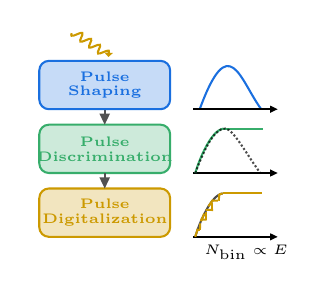
\begin{tikzpicture}[x=0.75pt,y=0.75pt,yscale=-1,xscale=1]
%uncomment if require: \path (0,623);
%set diagram left start at 0, and has height of 623
%Curve Lines [id:da31175352604231354]
\draw [color={rgb, 255:red, 26; green, 111; blue, 223 } ,draw opacity=1 ] (297.29,228.67) .. controls (311.48,189.89) and (316.58,214.56) .. (326.94,228.67) ;
%Straight Lines [id:da8734375505712497]
\draw (294.07,228.67) -- (331.84,228.67) ;
\draw [shift={(334.84,228.67)}, rotate = 180] [fill={rgb, 255:red, 0; green, 0; blue, 0 } ][line width=0.08] [draw opacity=0] (3.57,-1.72) -- (0,0) -- (3.57,1.72) -- cycle ;
%Straight Lines [id:da44513384727711636]
\draw (294.07,290.16) -- (331.84,290.16) ;
\draw [shift={(334.84,290.16)}, rotate = 180] [fill={rgb, 255:red, 0; green, 0; blue, 0 } ][line width=0.08] [draw opacity=0] (3.57,-1.72) -- (0,0) -- (3.57,1.72) -- cycle ;
%Curve Lines [id:da06577028557977793]
\draw [color={rgb, 255:red, 0; green, 0; blue, 0 } ,draw opacity=0.7 ] (295.15,290.16) .. controls (296.85,284.16) and (302.58,269.99) .. (308.33,269.24) ;
%Straight Lines [id:da0572237289311508]
\draw [color={rgb, 255:red, 0; green, 0; blue, 0 } ,draw opacity=0.7 ] (308.33,269.24) -- (327.15,269.24) ;
%Curve Lines [id:da3804043288541633]
\draw [color={rgb, 255:red, 204; green, 153; blue, 0 } ,draw opacity=1 ] [dash pattern={on 3pt off 3pt on 3pt off 3pt}] (295.15,290.16) .. controls (296.85,284.16) and (302.58,269.99) .. (308.33,269.24) ;
%Straight Lines [id:da5333998307295363]
\draw [color={rgb, 255:red, 204; green, 153; blue, 0 } ,draw opacity=1 ] (295.76,286.75) -- (297.39,286.83) ;
%Straight Lines [id:da40393427405433224]
\draw [color={rgb, 255:red, 204; green, 153; blue, 0 } ,draw opacity=1 ] (297.39,286.83) -- (297.49,283.65) ;
%Straight Lines [id:da7440185216718632]
\draw [color={rgb, 255:red, 204; green, 153; blue, 0 } ,draw opacity=1 ] (303.28,272.68) -- (305.99,272.69) ;
%Straight Lines [id:da4575813772961881]
\draw [color={rgb, 255:red, 204; green, 153; blue, 0 } ,draw opacity=1 ] (306.47,272.78) -- (306.7,269.62) ;
%Straight Lines [id:da012864593156911797]
\draw [color={rgb, 255:red, 204; green, 153; blue, 0 } ,draw opacity=1 ] (297.68,281.8) -- (300.65,281.85) ;
%Straight Lines [id:da7563678124476333]
\draw [color={rgb, 255:red, 204; green, 153; blue, 0 } ,draw opacity=1 ] (300.13,281.96) -- (300.13,278.31) ;
%Straight Lines [id:da5333243365793827]
\draw [color={rgb, 255:red, 204; green, 153; blue, 0 } ,draw opacity=1 ] (301,277.21) -- (300.2,277.18) -- (303.71,277.22) ;
%Straight Lines [id:da6175946543817453]
\draw [color={rgb, 255:red, 204; green, 153; blue, 0 } ,draw opacity=1 ] (303.06,277.27) -- (303.06,276.8) -- (303.06,276.78) -- (303.06,273.62) ;
%Straight Lines [id:da3521344691026579]
\draw [color={rgb, 255:red, 204; green, 153; blue, 0 } ,draw opacity=1 ] (308.33,269.24) -- (327.15,269.24) ;
%Shape: Wave [id:dp9368433800430482]
\draw [color={rgb, 255:red, 204; green, 153; blue, 0 } ,draw opacity=1 ] (235.61,192.06) .. controls (235.39,192.63) and (235.3,193.09) .. (235.56,193.27) .. controls (235.94,193.52) and (237.01,193.07) .. (238.13,192.59) .. controls (239.24,192.11) and (240.31,191.66) .. (240.7,191.91) .. controls (241.08,192.17) and (240.68,193.07) .. (240.25,194.02) .. controls (239.83,194.96) and (239.43,195.86) .. (239.81,196.12) .. controls (240.2,196.38) and (241.26,195.92) .. (242.38,195.45) .. controls (243.5,194.97) and (244.57,194.51) .. (244.95,194.77) .. controls (245.34,195.03) and (244.94,195.93) .. (244.51,196.87) .. controls (244.09,197.82) and (243.68,198.72) .. (244.07,198.98) .. controls (244.45,199.24) and (245.52,198.78) .. (246.64,198.3) .. controls (247.76,197.82) and (248.82,197.37) .. (249.21,197.63) .. controls (249.59,197.88) and (249.19,198.78) .. (248.77,199.73) .. controls (248.34,200.67) and (247.94,201.58) .. (248.33,201.83) .. controls (248.71,202.09) and (249.78,201.64) .. (250.9,201.16) .. controls (252.01,200.68) and (253.08,200.22) .. (253.47,200.48) .. controls (253.82,200.72) and (253.51,201.51) .. (253.12,202.37) ;
%Shape: Triangle [id:dp9985044017508556]
\draw [color={rgb, 255:red, 204; green, 153; blue, 0 } ,draw opacity=1 ][fill={rgb, 255:red, 204; green, 153; blue, 0 } ,fill opacity=1 ] (253.35,202.81) -- (252.57,201.95) -- (254.24,202.02) -- cycle ;
%Rounded Rect [id:dp19934922796405263]
\draw [color={rgb, 255:red, 55; green, 173; blue, 107 } ,draw opacity=1 ][fill={rgb, 255:red, 55; green, 173; blue, 107 } ,fill opacity=0.25 ] (220,240.78) .. controls (220,238.21) and (222.09,236.12) .. (224.66,236.12) -- (278.38,236.12) .. controls (280.95,236.12) and (283.04,238.21) .. (283.04,240.78) -- (283.04,254.76) .. controls (283.04,257.33) and (280.95,259.42) .. (278.38,259.42) -- (224.66,259.42) .. controls (222.09,259.42) and (220,257.33) .. (220,254.76) -- cycle ;
%Straight Lines [id:da15405365263406912]
\draw [color={rgb, 255:red, 81; green, 81; blue, 81 } ,draw opacity=1 ] (251.52,228.67) -- (251.52,233.12) ;
\draw [shift={(251.52,236.12)}, rotate = 270] [fill={rgb, 255:red, 81; green, 81; blue, 81 } ,fill opacity=1 ][line width=0.08] [draw opacity=0] (5.36,-2.57) -- (0,0) -- (5.36,2.57) -- cycle ;
%Rounded Rect [id:dp9679678320320008]
\draw [color={rgb, 255:red, 26; green, 111; blue, 223 } ,draw opacity=1 ][fill={rgb, 255:red, 26; green, 111; blue, 223 } ,fill opacity=0.25 ] (220,210.03) .. controls (220,207.46) and (222.09,205.37) .. (224.66,205.37) -- (278.38,205.37) .. controls (280.95,205.37) and (283.04,207.46) .. (283.04,210.03) -- (283.04,224.01) .. controls (283.04,226.58) and (280.95,228.67) .. (278.38,228.67) -- (224.66,228.67) .. controls (222.09,228.67) and (220,226.58) .. (220,224.01) -- cycle ;
%Rounded Rect [id:dp4047477037578918]
\draw [color={rgb, 255:red, 204; green, 153; blue, 0 } ,draw opacity=1 ][fill={rgb, 255:red, 204; green, 153; blue, 0 } ,fill opacity=0.25 ] (220,271.53) .. controls (220,268.96) and (222.09,266.87) .. (224.66,266.87) -- (278.38,266.87) .. controls (280.95,266.87) and (283.04,268.96) .. (283.04,271.53) -- (283.04,285.51) .. controls (283.04,288.08) and (280.95,290.16) .. (278.38,290.16) -- (224.66,290.16) .. controls (222.09,290.16) and (220,288.08) .. (220,285.51) -- cycle ;
%Straight Lines [id:da0010432308854115835]
\draw (294.07,259.42) -- (331.84,259.42) ;
\draw [shift={(334.84,259.42)}, rotate = 180] [fill={rgb, 255:red, 0; green, 0; blue, 0 } ][line width=0.08] [draw opacity=0] (3.57,-1.72) -- (0,0) -- (3.57,1.72) -- cycle ;
%Curve Lines [id:da4874347648440388]
\draw [color={rgb, 255:red, 55; green, 173; blue, 107 } ,draw opacity=1 ] (295.17,259.42) .. controls (296.91,253.15) and (302.75,238.82) .. (308.61,238.06) ;
%Straight Lines [id:da23704226954075758]
\draw [color={rgb, 255:red, 55; green, 173; blue, 107 } ,draw opacity=1 ] (308.61,238.06) -- (327.80,238.06) ;
%Curve Lines [id:da042698988524645376]
\draw [color={rgb, 255:red, 0; green, 0; blue, 0 } ,draw opacity=0.7 ] [dash pattern={on 0.75pt off 0.75pt on 0.75pt off 0.75pt}] (295.17,259.42) .. controls (301.17,243.29) and (305.64,237.91) .. (309.53,237.99) .. controls (313.43,238.08) and (319.93,250.52) .. (326.49,259.42) ;
%Straight Lines [id:da33392936363629766]
\draw [color={rgb, 255:red, 81; green, 81; blue, 81 } ,draw opacity=1 ] (251.52,259.42) -- (251.52,263.87) ;
\draw [shift={(251.52,266.87)}, rotate = 270] [fill={rgb, 255:red, 81; green, 81; blue, 81 } ,fill opacity=1 ][line width=0.08] [draw opacity=0] (5.36,-2.57) -- (0,0) -- (5.36,2.57) -- cycle ;
% Text Node
\draw (298.00,292.60) node [anchor=north west][inner sep=0.75pt] [font=\tiny] [align=left] {$N_{\mathrm{bin}} \propto E$};
% Text Node
\draw (251.52,247.77) node [anchor=center, align=center, font=\fontsize{4.5}{5.4}\selectfont\bfseries, color={rgb, 255:red, 55; green, 173; blue, 107 }] {Pulse\\Discrimination};
% Text Node
\draw (251.52,217.02) node [anchor=center, align=center, font=\fontsize{4.5}{5.4}\selectfont\bfseries, color={rgb, 255:red, 26; green, 111; blue, 223 }] {Pulse\\Shaping};
% Text Node
\draw (251.52,278.51) node [anchor=center, align=center, font=\fontsize{4.5}{5.4}\selectfont\bfseries, color={rgb, 255:red, 204; green, 153; blue, 0 }] {Pulse\\Digitalization}; 


% Optional: label the incoming photon next to the yellow squiggle.
% Uncomment the next line if you want it.
%\draw (236.50,191.00) node [anchor=south east, font=\fontsize{4.5}{5.4}\selectfont, color={rgb, 255:red, 204; green, 153; blue, 0 }] {$h\nu$};
\end{tikzpicture}
}
%  Needs only \usepackage{tikz}, which the poster already loads.
% =====================================================================

\tikzset{every picture/.style={line width=0.75pt}}
%set default line width to 0.75pt 
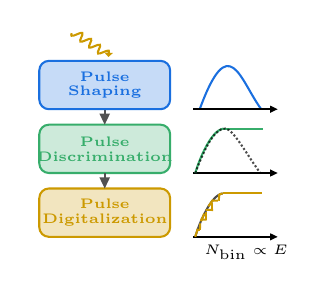
\begin{tikzpicture}[x=0.75pt,y=0.75pt,yscale=-1,xscale=1]
%uncomment if require: \path (0,623);
%set diagram left start at 0, and has height of 623
%Curve Lines [id:da31175352604231354]
\draw [color={rgb, 255:red, 26; green, 111; blue, 223 } ,draw opacity=1 ] (297.29,228.67) .. controls (311.48,189.89) and (316.58,214.56) .. (326.94,228.67) ;
%Straight Lines [id:da8734375505712497]
\draw (294.07,228.67) -- (331.84,228.67) ;
\draw [shift={(334.84,228.67)}, rotate = 180] [fill={rgb, 255:red, 0; green, 0; blue, 0 } ][line width=0.08] [draw opacity=0] (3.57,-1.72) -- (0,0) -- (3.57,1.72) -- cycle ;
%Straight Lines [id:da44513384727711636]
\draw (294.07,290.16) -- (331.84,290.16) ;
\draw [shift={(334.84,290.16)}, rotate = 180] [fill={rgb, 255:red, 0; green, 0; blue, 0 } ][line width=0.08] [draw opacity=0] (3.57,-1.72) -- (0,0) -- (3.57,1.72) -- cycle ;
%Curve Lines [id:da06577028557977793]
\draw [color={rgb, 255:red, 0; green, 0; blue, 0 } ,draw opacity=0.7 ] (295.15,290.16) .. controls (296.85,284.16) and (302.58,269.99) .. (308.33,269.24) ;
%Straight Lines [id:da0572237289311508]
\draw [color={rgb, 255:red, 0; green, 0; blue, 0 } ,draw opacity=0.7 ] (308.33,269.24) -- (327.15,269.24) ;
%Curve Lines [id:da3804043288541633]
\draw [color={rgb, 255:red, 204; green, 153; blue, 0 } ,draw opacity=1 ] [dash pattern={on 3pt off 3pt on 3pt off 3pt}] (295.15,290.16) .. controls (296.85,284.16) and (302.58,269.99) .. (308.33,269.24) ;
%Straight Lines [id:da5333998307295363]
\draw [color={rgb, 255:red, 204; green, 153; blue, 0 } ,draw opacity=1 ] (295.76,286.75) -- (297.39,286.83) ;
%Straight Lines [id:da40393427405433224]
\draw [color={rgb, 255:red, 204; green, 153; blue, 0 } ,draw opacity=1 ] (297.39,286.83) -- (297.49,283.65) ;
%Straight Lines [id:da7440185216718632]
\draw [color={rgb, 255:red, 204; green, 153; blue, 0 } ,draw opacity=1 ] (303.28,272.68) -- (305.99,272.69) ;
%Straight Lines [id:da4575813772961881]
\draw [color={rgb, 255:red, 204; green, 153; blue, 0 } ,draw opacity=1 ] (306.47,272.78) -- (306.7,269.62) ;
%Straight Lines [id:da012864593156911797]
\draw [color={rgb, 255:red, 204; green, 153; blue, 0 } ,draw opacity=1 ] (297.68,281.8) -- (300.65,281.85) ;
%Straight Lines [id:da7563678124476333]
\draw [color={rgb, 255:red, 204; green, 153; blue, 0 } ,draw opacity=1 ] (300.13,281.96) -- (300.13,278.31) ;
%Straight Lines [id:da5333243365793827]
\draw [color={rgb, 255:red, 204; green, 153; blue, 0 } ,draw opacity=1 ] (301,277.21) -- (300.2,277.18) -- (303.71,277.22) ;
%Straight Lines [id:da6175946543817453]
\draw [color={rgb, 255:red, 204; green, 153; blue, 0 } ,draw opacity=1 ] (303.06,277.27) -- (303.06,276.8) -- (303.06,276.78) -- (303.06,273.62) ;
%Straight Lines [id:da3521344691026579]
\draw [color={rgb, 255:red, 204; green, 153; blue, 0 } ,draw opacity=1 ] (308.33,269.24) -- (327.15,269.24) ;
%Shape: Wave [id:dp9368433800430482]
\draw [color={rgb, 255:red, 204; green, 153; blue, 0 } ,draw opacity=1 ] (235.61,192.06) .. controls (235.39,192.63) and (235.3,193.09) .. (235.56,193.27) .. controls (235.94,193.52) and (237.01,193.07) .. (238.13,192.59) .. controls (239.24,192.11) and (240.31,191.66) .. (240.7,191.91) .. controls (241.08,192.17) and (240.68,193.07) .. (240.25,194.02) .. controls (239.83,194.96) and (239.43,195.86) .. (239.81,196.12) .. controls (240.2,196.38) and (241.26,195.92) .. (242.38,195.45) .. controls (243.5,194.97) and (244.57,194.51) .. (244.95,194.77) .. controls (245.34,195.03) and (244.94,195.93) .. (244.51,196.87) .. controls (244.09,197.82) and (243.68,198.72) .. (244.07,198.98) .. controls (244.45,199.24) and (245.52,198.78) .. (246.64,198.3) .. controls (247.76,197.82) and (248.82,197.37) .. (249.21,197.63) .. controls (249.59,197.88) and (249.19,198.78) .. (248.77,199.73) .. controls (248.34,200.67) and (247.94,201.58) .. (248.33,201.83) .. controls (248.71,202.09) and (249.78,201.64) .. (250.9,201.16) .. controls (252.01,200.68) and (253.08,200.22) .. (253.47,200.48) .. controls (253.82,200.72) and (253.51,201.51) .. (253.12,202.37) ;
%Shape: Triangle [id:dp9985044017508556]
\draw [color={rgb, 255:red, 204; green, 153; blue, 0 } ,draw opacity=1 ][fill={rgb, 255:red, 204; green, 153; blue, 0 } ,fill opacity=1 ] (253.35,202.81) -- (252.57,201.95) -- (254.24,202.02) -- cycle ;
%Rounded Rect [id:dp19934922796405263]
\draw [color={rgb, 255:red, 55; green, 173; blue, 107 } ,draw opacity=1 ][fill={rgb, 255:red, 55; green, 173; blue, 107 } ,fill opacity=0.25 ] (220,240.78) .. controls (220,238.21) and (222.09,236.12) .. (224.66,236.12) -- (278.38,236.12) .. controls (280.95,236.12) and (283.04,238.21) .. (283.04,240.78) -- (283.04,254.76) .. controls (283.04,257.33) and (280.95,259.42) .. (278.38,259.42) -- (224.66,259.42) .. controls (222.09,259.42) and (220,257.33) .. (220,254.76) -- cycle ;
%Straight Lines [id:da15405365263406912]
\draw [color={rgb, 255:red, 81; green, 81; blue, 81 } ,draw opacity=1 ] (251.52,228.67) -- (251.52,233.12) ;
\draw [shift={(251.52,236.12)}, rotate = 270] [fill={rgb, 255:red, 81; green, 81; blue, 81 } ,fill opacity=1 ][line width=0.08] [draw opacity=0] (5.36,-2.57) -- (0,0) -- (5.36,2.57) -- cycle ;
%Rounded Rect [id:dp9679678320320008]
\draw [color={rgb, 255:red, 26; green, 111; blue, 223 } ,draw opacity=1 ][fill={rgb, 255:red, 26; green, 111; blue, 223 } ,fill opacity=0.25 ] (220,210.03) .. controls (220,207.46) and (222.09,205.37) .. (224.66,205.37) -- (278.38,205.37) .. controls (280.95,205.37) and (283.04,207.46) .. (283.04,210.03) -- (283.04,224.01) .. controls (283.04,226.58) and (280.95,228.67) .. (278.38,228.67) -- (224.66,228.67) .. controls (222.09,228.67) and (220,226.58) .. (220,224.01) -- cycle ;
%Rounded Rect [id:dp4047477037578918]
\draw [color={rgb, 255:red, 204; green, 153; blue, 0 } ,draw opacity=1 ][fill={rgb, 255:red, 204; green, 153; blue, 0 } ,fill opacity=0.25 ] (220,271.53) .. controls (220,268.96) and (222.09,266.87) .. (224.66,266.87) -- (278.38,266.87) .. controls (280.95,266.87) and (283.04,268.96) .. (283.04,271.53) -- (283.04,285.51) .. controls (283.04,288.08) and (280.95,290.16) .. (278.38,290.16) -- (224.66,290.16) .. controls (222.09,290.16) and (220,288.08) .. (220,285.51) -- cycle ;
%Straight Lines [id:da0010432308854115835]
\draw (294.07,259.42) -- (331.84,259.42) ;
\draw [shift={(334.84,259.42)}, rotate = 180] [fill={rgb, 255:red, 0; green, 0; blue, 0 } ][line width=0.08] [draw opacity=0] (3.57,-1.72) -- (0,0) -- (3.57,1.72) -- cycle ;
%Curve Lines [id:da4874347648440388]
\draw [color={rgb, 255:red, 55; green, 173; blue, 107 } ,draw opacity=1 ] (295.17,259.42) .. controls (296.91,253.15) and (302.75,238.82) .. (308.61,238.06) ;
%Straight Lines [id:da23704226954075758]
\draw [color={rgb, 255:red, 55; green, 173; blue, 107 } ,draw opacity=1 ] (308.61,238.06) -- (327.80,238.06) ;
%Curve Lines [id:da042698988524645376]
\draw [color={rgb, 255:red, 0; green, 0; blue, 0 } ,draw opacity=0.7 ] [dash pattern={on 0.75pt off 0.75pt on 0.75pt off 0.75pt}] (295.17,259.42) .. controls (301.17,243.29) and (305.64,237.91) .. (309.53,237.99) .. controls (313.43,238.08) and (319.93,250.52) .. (326.49,259.42) ;
%Straight Lines [id:da33392936363629766]
\draw [color={rgb, 255:red, 81; green, 81; blue, 81 } ,draw opacity=1 ] (251.52,259.42) -- (251.52,263.87) ;
\draw [shift={(251.52,266.87)}, rotate = 270] [fill={rgb, 255:red, 81; green, 81; blue, 81 } ,fill opacity=1 ][line width=0.08] [draw opacity=0] (5.36,-2.57) -- (0,0) -- (5.36,2.57) -- cycle ;
% Text Node
\draw (298.00,292.60) node [anchor=north west][inner sep=0.75pt] [font=\tiny] [align=left] {$N_{\mathrm{bin}} \propto E$};
% Text Node
\draw (251.52,247.77) node [anchor=center, align=center, font=\fontsize{4.5}{5.4}\selectfont\bfseries, color={rgb, 255:red, 55; green, 173; blue, 107 }] {Pulse\\Discrimination};
% Text Node
\draw (251.52,217.02) node [anchor=center, align=center, font=\fontsize{4.5}{5.4}\selectfont\bfseries, color={rgb, 255:red, 26; green, 111; blue, 223 }] {Pulse\\Shaping};
% Text Node
\draw (251.52,278.51) node [anchor=center, align=center, font=\fontsize{4.5}{5.4}\selectfont\bfseries, color={rgb, 255:red, 204; green, 153; blue, 0 }] {Pulse\\Digitalization}; 


% Optional: label the incoming photon next to the yellow squiggle.
% Uncomment the next line if you want it.
%\draw (236.50,191.00) node [anchor=south east, font=\fontsize{4.5}{5.4}\selectfont, color={rgb, 255:red, 204; green, 153; blue, 0 }] {$h\nu$};
\end{tikzpicture}
